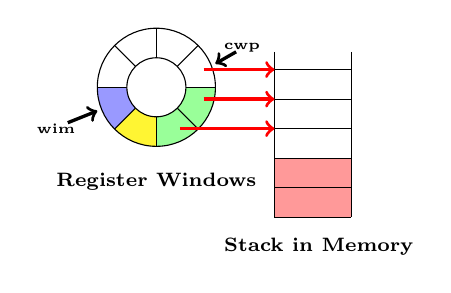
\begin{tikzpicture}[scale=0.75]
    \fill[green!40!white] (0,0) -- (0,-1cm) arc (-90:0:1cm) -- (0,0);
    % \fill[blue!40!white] (0,0) -- (0,-1cm) arc (-90:-135:1cm) -- (0,0);
    \fill[yellow!80!white] (0,0) -- (0,-1cm) arc (-90:-135:1cm) -- (0,0);
    \fill[blue!40!white] (0,0) -- (-1,0cm) arc (-180:-135:1cm) -- (0,0);
    \draw (0, 0) -- (90:1cm);
    \draw (0, 0) -- (45:1cm);
    \draw (0, 0) -- (0:1cm);
    \draw (0, 0) -- (-45:1cm);
    \draw (0, 0) -- (-90:1cm);
    \draw (0, 0) -- (-135:1cm);
    \draw (0, 0) -- (-180:1cm);
    \draw (0, 0) -- (135:1cm);
    \fill[white] (0, 0) circle (0.5cm);
    \draw (0, 0) circle (1cm);
    \draw (0, 0) circle (0.5cm);
    % \draw[very thick, blue] (0, -0.3) -- (0, -1.2);
    % \draw[very thick, blue] (0, -0.32) -- (0.1, -0.32);
    % \draw[very thick, blue] (0, -1.18) -- (0.1, -1.18);
    % \node(wim) at (-1.3, -1.1) {\tiny \bf wim};
    % \draw[->, very thick] (-1, -1.1) -- (-0.5, -0.9);

    \node(wim) at (-1.7, -0.7) {\tiny \bf wim};
    \draw[->, very thick] (-1.5, -0.6) -- (-1, -0.4);
    

    \node(cwp) at (1.45, 0.67) {\tiny \bf cwp};
    \draw[->, very thick] (1.35, 0.6) -- (1, 0.4);

    \node(regwin) at (0, -1.6) {\scriptsize \bf Register Windows};

    %%%%%%%%%%%%%%%%%%%%%%%%%%%%%%%%%%%%%%%%%%%%%%%%%%%%%%

    \fill[red!40!white] (2, -1.2) rectangle (3.3, -1.7);
    \fill[red!40!white] (2, -1.7) rectangle (3.3, -2.2);

    \draw[-] (2, 0.6) -- (2, -2.2);
    \draw[-] (3.3, 0.6) -- (3.3, -2.2);
    
    \draw[-] (2, 0.3) -- (3.3, 0.3);
    \draw[-] (2, -0.2) -- (3.3, -0.2);
    \draw[-] (2, -0.7) -- (3.3, -0.7);
    \draw[-] (2, -1.2) -- (3.3, -1.2);
    \draw[-] (2, -1.7) -- (3.3, -1.7);
    \draw[-] (2, -2.2) -- (3.3, -2.2);

    \node(stkfm) at (2.75, -2.7) {\scriptsize \bf Stack in Memory};

    %%%%%%%%%%%%%%%%%%%%%%%%%%%%%%%%%%%%%%%%%%%%%%%%%%%%%%%

    \draw[->, very thick, red] (0.8, 0.3) -- (2, 0.3);
    \draw[->, very thick, red] (0.8, -0.2) -- (2, -0.2);
    \draw[->, very thick, red] (0.4, -0.7) -- (2, -0.7);

    %%%%%%%%%%%%%%%%%%%%%%%%%%%%%%%%%%%%%%%%%%%%%%%%%%%%%%

    % \node(abstract) at (4.7, -0.2) {$\xLongrightarrow{\text{Abstract}}$};

    %%%%%%%%%%%%%%%%%%%%%%%%%%%%%%%%%%%%%%%%%%%%%%%%%%%%%%
\end{tikzpicture} 